\documentclass[main]{subfiles}
\begin{document}

%@@@@@@@@@@@@@@@@@@@@@@@@@@@@@@
% Main Topics: Nervous System Organization - 27.09.2018
% Lecturer: Wolfger von der Behrens
% author: Vanessa Leite - base document from benelot/eth-intro-to-neuroinformatics-summary

\section{Nervous System Organization}
\subsection{Anatomy}
\begin{itemize}[noitemsep,nolistsep]
	\item Central nervous system (CNS): Brain and spinal cord.
	\item Peripheral nervous system (PNS): Somatic, autonomic (sympathetic and parasympathetic) NS.
	\item Brain cuts: Horizontal plane cut, coronal/frontal cut and sagittal cut (between eyes). Cross-section through spinal cord, for example.
	\item The skull protects, meninges envelope the CNS and has 3 layers, the dura mater, arachnoid mater and pia mater. Primary function is protection.
	\item The cortex is the layer directly under the surface of the brain.
	\item There are 4 lobes in each hemisphere. Lobes are separated by fissures in the cortex.
\end{itemize}
\begin{figure}[H]
	\centering
	\begin{subfigure}[b]{0.5\textwidth}
		\centering
		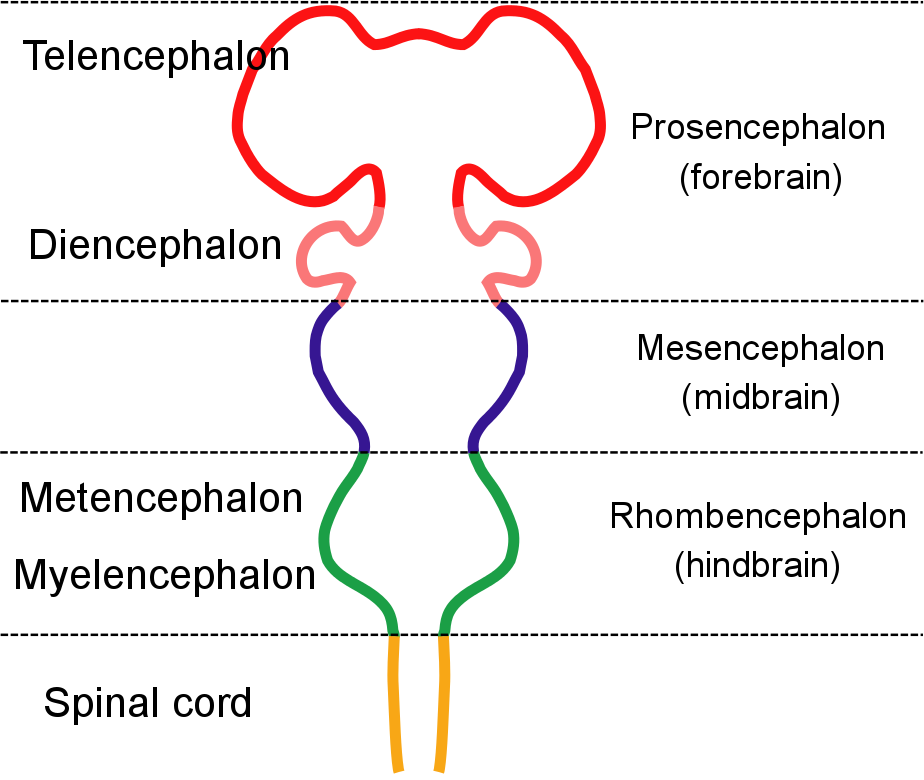
\includegraphics[width=\textwidth]{brain-parts.png}
	\end{subfigure}%
	~
	\begin{subfigure}[b]{0.5\textwidth}
		\centering
		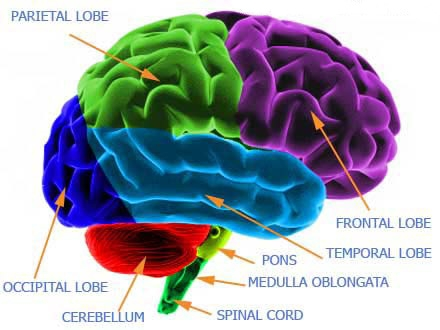
\includegraphics[width=\textwidth]{brain.png}
	\end{subfigure}
\end{figure}
\begin{figure}[H]
	\centering
	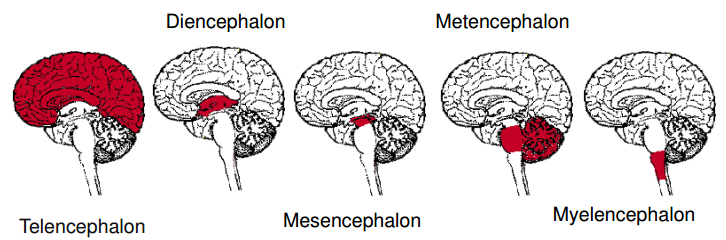
\includegraphics[width=\textwidth]{brain_anatomy_01.png}
\end{figure}
\begin{figure}[H]
	\centering
	\begin{subfigure}[b]{0.5\textwidth}
		\centering
		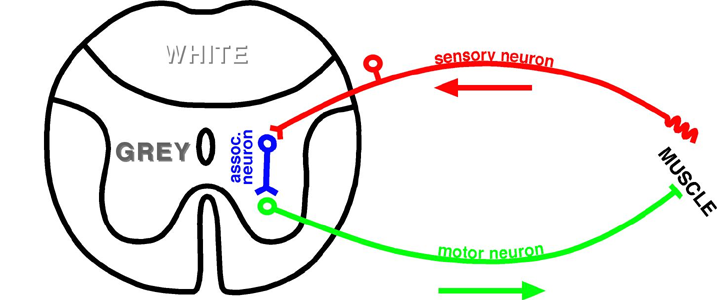
\includegraphics[width=\textwidth]{motor-sensory-neuron.png}
	\end{subfigure}%
	~
	\begin{subfigure}[b]{0.5\textwidth}
		\centering
		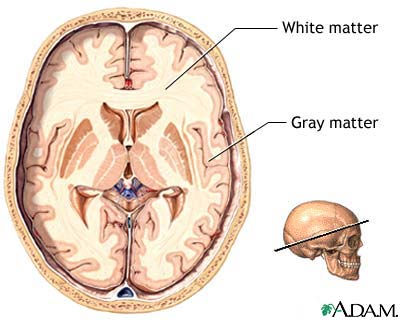
\includegraphics[width=\textwidth]{brain-cut.png}
	\end{subfigure}
\end{figure}

\subsection{Building elements of the brain}
\begin{itemize}[noitemsep,nolistsep]
	\item Forebrain (Prosencephalon): Cortex, thalamus, hippocampus, basal ganglia, corpus callosum.
	\item Midbrain (Mesencephalon): Tectum, tegmentum.
	\item Hindbrain (Rhombencephalon): Cerebellum, pons, medulla oblongata.
	\item White matter: Glia cells, myelinated axons.
	\item Grey matter: Neurons (soma).
	\item Neocortex: Six-layered cortex that forms the surface of most of the cerebral hemispheres.
	\item Corpus callosum: Midline fiber bundle, connects the two cerebral hemispheres.
	\item Gyrus: Ridges of the cotex, with valleys (sulci).
\end{itemize}
\subsubsection{The limbic system}
\begin{itemize}[noitemsep,nolistsep]
	\item Structure: On medial and basal surfaces of cerebral hemispheres.
	\item Includes cingulate gyrus, parahippocampal gyrus, hippocampal formation, fornix, amygdala, septum, mamillary bodies
	\item Function: Emotional expression, memory acquisition, fear conditioning, violence and aggression.
\end{itemize}
\begin{figure}[H]
	\centering
	\begin{subfigure}[b]{0.5\textwidth}
		\centering
		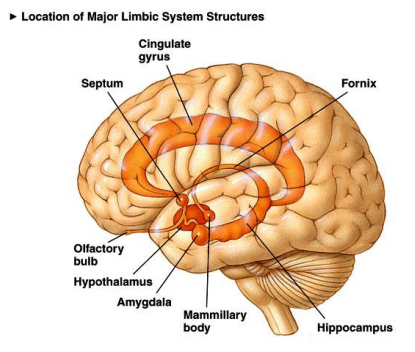
\includegraphics[width=\textwidth]{brain_anatomy_02.png}
	\end{subfigure}%
	~
	\begin{subfigure}[b]{0.5\textwidth}
		\centering
		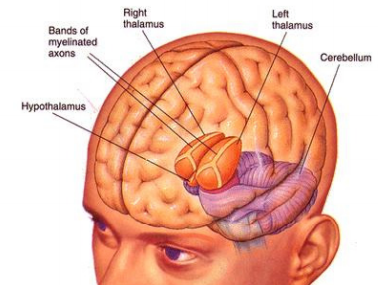
\includegraphics[width=\textwidth]{brain_anatomy_03.png}
	\end{subfigure}
\end{figure}
\subsubsection{Hypothalamus and thalamus}
\begin{itemize}[noitemsep,nolistsep]
	\item Structure: Relatively large, two symmetric large nuclei, many projections.
	\item Function: Relay station, domain-specific information processing.
	\item The upper brain stem is the diencephalon.
	\item The hypothalamus is very small and controls autonomic mechanisms.
\end{itemize}
\subsubsection{Basal ganglia}
\begin{itemize}[noitemsep,nolistsep]
	\item Structure: Collection of nuclei embedded deep within the cortex.
	\item Partially surrounds the thalamus.
	\item Sensory projectons to the cerebrum
	\item Function: Regulate voluntary movement.
	\item Movement disorders like Parkinson's.
\end{itemize}
\subsubsection{Cerebellum}
\begin{itemize}[noitemsep,nolistsep]
	\item Structure: ``little brain'', has layered appearance and symmetry.
	\item Two hemispheres are connected by the vermis.
	\item Function: Coordinated motor behavior, posture adjustments and stores memories for simple learned motor responses.
\end{itemize}
\subsubsection{Reticular Formation}
\begin{itemize}[noitemsep,nolistsep]
	\item Structure: Diffuse arrangement of ascending and descending neurons.
	\item Function: Arousal, selective attention, respiration.
\end{itemize}
\subsubsection{Connections}
\begin{itemize}[noitemsep,nolistsep]
	\item The Basal ganglia projects to the cerebral cortex (via thalamus).
	\item The cerebellum projects to the cerebral cortex (via thalamus).
	\item The cerebral cortex projects to basal ganglia, cerebellum and motor neurons (and interneurons) via  pons.
\end{itemize}
\begin{figure}[H]
	\centering
	\begin{subfigure}[b]{0.5\textwidth}
		\centering
		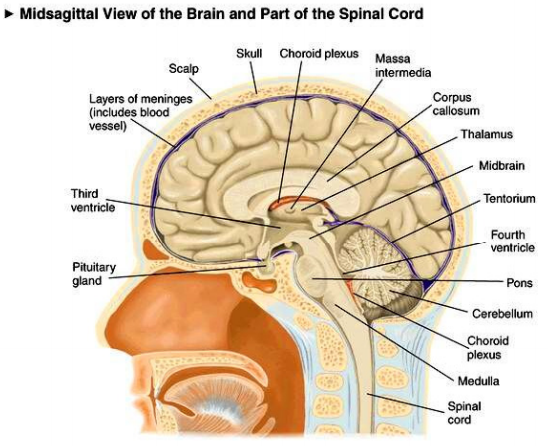
\includegraphics[width=\textwidth]{brain_anatomy_04.png}
	\end{subfigure}%
	~
	\begin{subfigure}[b]{0.5\textwidth}
		\centering
		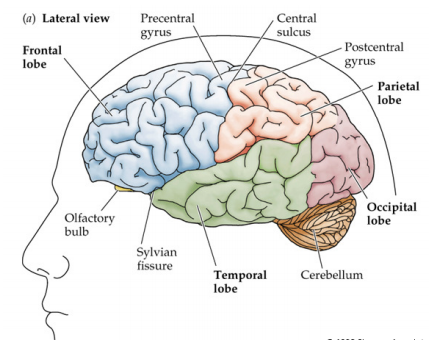
\includegraphics[width=\textwidth]{brain_anatomy_05.png}
	\end{subfigure}
\end{figure}

\subsection{Nervous system in numbers}
\begin{itemize}[noitemsep,nolistsep]
	\item $1\,mm^3$ of white matter is $9\,m$ of axons.
	\item $1\,mm^3$ of grey matter is $50'000$ neurons.
	\item In $1\,mm^3$ about $100'000$ cells.
	\item The cortex has six layers.
\end{itemize}

\subsection{Basic structure of the neuron}
\subsubsection{Components}
\begin{itemize}[noitemsep,nolistsep]
	\item Cell body
	\item Nucleus
	\item Dendrite: Input component.
	\item Axon: Output component, makes contact to other neurons.
	\item Myelin: Wraps around axons, makes white matter white.
	\item Boutons: At the ends of the axons, connects neurons.
	\item Soma: Body of a cell without it's extensions.
	\item Afferent: Neurons that carry nerve impulses from receptors to the CNS.
	\item Efferent: Neurons that carry information away from the CNS.
	\item Projection neuron: Neuron with long axons that project to distant targets.
\end{itemize}
\subsubsection{Axon transport}
\begin{itemize}[noitemsep,nolistsep]
	\item Golgi apparatus sits at the cell body.
	\item Transport of vesicles to the axon terminal (anterograde).
	\item Transport of empty vesicles back to the cell body (retrograde).
\end{itemize}
\subsubsection{Synapse}
\begin{itemize}[noitemsep,nolistsep]
	\item Boutons: connection point.
	\item Cleft: Little gap between presynaptic and postsynaptic neuron.
	\item Dendritic spines: Dendritic part of the synapse.
	\item Transmitter: Gets released by the presynaptic neuron, in vesicles.
	\item Vesicles: Transport the transmitter inside the cell.
	\item Receptors: Binding site for the transmitter.
\end{itemize}

\subsection{Muscle reflex and antagonistis}
\subsubsection{Reciprocal innervation of antagonistic muscles}
\begin{enumerate}[noitemsep,nolistsep]
	\item A tack produces a burst of firing (sensory neurons, for example on the finger).
	\item The burst excites excitatory spinal interneurons, which then excite the motor neurons of a muscle.
	\item The burst also excites inhibitory spinal interneurons that inhibit antagonist muscle motor neurons.
	\item One muscle gets contracted, the other relaxed, allowing for a rapid flexion. No brain involved (but gets informed).
\end{enumerate}
\subsubsection{Elicitation of a stretch reflex}
\begin{itemize}[noitemsep,nolistsep]
	\item When hitting the knee tendon with a hammer, the spindles of the thigh muscle get stretched and this elicits a burst of firing in the spindle afferents.
	\item The burst triggers a burst of firing in the thigh muscle motor neurons, causing contraction.
\end{itemize}



\end{document}
